\documentclass[article,type=msc,colorback,12pt,accentcolor=tud1d]{tudthesis}
\usepackage{ngerman}
\usepackage[english]{babel}
\usepackage{csquotes}
\MakeOuterQuote{"}
\usepackage{xcolor,colortbl}

\usepackage{titlesec}
\titleformat{\section}
{\normalfont\fontsize{20}{25}\bfseries}{\thesection}{1em}{}
 
\usepackage{hyperref}
\hypersetup{
	colorlinks,
	citecolor=blue,
	filecolor=blue,
	linkcolor=blue,
	urlcolor=blue
}
\usepackage{cite}

\graphicspath{ {img/} }

\newcommand{\getmydate}{%
  \ifcase\month%
    \or Januar\or Februar\or M\"arz%
    \or April\or Mai\or Juni\or Juli%
    \or August\or September\or Oktober%
    \or November\or Dezember%
  \fi\ \number\year%
}
\pdfmapfile{=5ch.map}
\pdfmapfile{=5fp.map}
\pdfmapfile{=5sf.map}

\begin{document}
  \thesistitle{Balanced Geohash Partitioning and Ef{}f{}icient Retrieval of Geospatial Big Data on Distributed and Parallel Platforms (Apache Spark)}
	{}
  \author{Hariharan Gandhi}
  \birthplace{Darmstadt}
  \referee{Prof. Alejandro Buchmann, Robert Rehner M.Sc [TU Darmstadt] }{Dr. Gregor Moehler, Dr. Raghu Kiran Ganti [IBM Research \& Development]}
  \department{\includegraphics[width=0.95\linewidth]{a} \\Databases and Distributed Systems}
  \group{Department of Computer Science \\Technical University of Darmstadt}
  
  \dateofexam{\today}{\today}
  \tuprints{12345}{1234}
  \makethesistitle
  \affidavit{Hariharan Gandhi}


\begin{abstract}
			
		 \hfill 	
		
		  \par Amongst several big data disciplines, \textit{spatial data} is one of the most exponentially proliferating data type. This could be attributed to the explosive increase in the number of users of mobile devices with sophisticated GPS\footnote{Global Positioning System} location sensors, emergence of social media and advancement in weather and navigation systems. More and more applications and businesses are providing location based services, personalised suggestions and most disruptive apps of recent times, such as Uber for taxi services, AirBnB for resource sharing, Google Maps, geo-tagged Tweets, Instagram photos, drones, logistics, weather apps, all provide location aware service to their users.
		    \\ \\
		  Exploiting this Geospatial dimension of information for the benefits of analytics is interesting and challenging. To store and process such huge volumes of data, we harness the efficiency of emerging distributed and parallel computing platforms, such as \textit{\textbf{Apache Spark, Hadoop Mapreduce, Hadoop Distributed Files Systems}}. However, conventional distributed storage and processing systems, do not provide native support for handling and efficiently storing Geospatial data types. The challenge is further made intricate by the necessity to preserve data points' locality in order to minimize network cost involved due to shuffling of intermittent results between the computing nodes. In this thesis work, we use the large scale data processing engine, \textbf{Apache Spark }\cite{sparkmainpaper}, to process Geospatial datasets. Spark provides \textit{resilient distributed dataset} (RDD)\cite{RDDmainpaper}, which is a collection of dataset partitioned across the nodes of a cluster for parallel operation \cite{sparkHomePage}. 
		   \\ \\
		  Geospatial operations such as \textit{contains, within, overlaps} etc involves a shuffling between partitions when there is a scan for data points in a region. This means that geographically closer data points should be preserved in the same partitions within a Spark RDD for reduced shuffling, minimal network cost, and efficient scans and retrieval. Spark's default partitioning are \textit{Range-based and Hash-based}(Java Hashcode) both of which are not suitable for achieving spatial locality within partitions. It emphasizes the need for developing a 'custom' Geospatial partitioning and retrieval methodology tailored to store and retrieve the overwhelming amount of Geospatial big data. 
		 \\ \\
		  This thesis works aims at addressing this issue by proposing and providing a geographically load balanced partitioning mechanism, for Apache Spark, tailored for Geospatial dataset and further by providing an optimized querying layer for efficient retrieval of records on spatial queries. Experimental results, using New York Taxi dataset, show  improvement in data points' locality for minimized shuffling and efficiency with scanning and retrieving results for spatial queries in terms of response time and number of records scanned.\cite{sparkbook}
		

\end{abstract}  

\clearpage


%=====INDEX================================================================================

\setlength{ \parskip }{1em}
\index{key}
\tableofcontents 
\cleardoublepage 

\listoffigures
\clearpage
\appendix
\cleardoublepage 

% abstract, acknowledgements, contents
	\hfill
  \section{Introduction}
  \hfill \break
 
		\subsection{Motivation}
		
		\par Of late, Geospatial data has seen an unprecedented growth rate owing to the increasing popularity of mobile devices. According to GSMA report 2016 \cite{GSMA_REPORT_2016}, there were \textbf{7.6 billion} mobile subscriptions with 4.7 'unique' subscribers by the end of 2015, one billion more expected by 2020 and more interestingly, more than half of the world's population has mobile subscriptions with a penetration rate of more than 63\% and operator revenue of one trillion dollars.
		
		These devices are equipped with sophisticated \textit{Global Positioning System(GPS)} which reports the exact location information of the device. This feature has made lives easier with tons of day to day applications providing \textit{location based services}. Some of these apps. such as maps, navigation, social networking, have become integral part of our lives. The major source of data for these applications originates from the users through opportunistic or participatory sensing. Besides mobile devices, almost every web application have also centralized their services to location based. Twitter trends in a particular city, traffic information for a city, weather forecast in a location/city - all involve spatial data associated with them. 
		
		With all these sudden burst in location data, comes the challenge of scalability and efficiency in processing these streams of data, and need for techniques that could efficiently process spatial queries.  Big data processing and management has been in practice for years now and are providing solutions to most of the world's big data needs. Several distributed file systems -\textit{ Hadoop Distributed File System(HDFS), Google File System(GFS)} and distributed processing engines and databases like \textit{Big Table, Hadoop, Spark} etc are in place to crunch the big data thrown at them. So, to handle our big-spatial-data, our obvious choice should be use of these distributed processing platforms. There are several spatial indexing techniques in spatial databases like \begin{itemize}
			\item Quadtrees, 
			\item Grid files, 
			\item R-trees
		\end{itemize}They are being used extensively to store and retrieve spatial data types in traditional Relational Database Management Systems(RDBMS). Several such approaches have also been proposed to use in big spatial data processing platforms like Hadoop MapReduce. Nonetheless, almost all of these approaches, demand certain level of modification to the internal implementation of their indexing schemes in these frameworks, hence leading to additional complexity. This would also result in  system specific approaches \cite{Lee:2014:ESQ:2666310.2666481} \cite{6691586}. 
		
		\clearpage
		There are also huge possibilities to scale these data processing clusters as they are increasingly available and accessible via Cloud Computing. Besides all these available big data processing engine, there is so simple solution to efficiently handle spatial data in these parallel platforms without modifying their internals. Also, their working cannot be optimized as long as location awareness is introduced into these systems and they are extended to handle spatial data. One major challenge in such cluster based engines is to minimize shuffling of data between nodes of a cluster thereby reducing the expense of network cost, minimizing the number of parallel tasks launched and processed, efficient and quicker query processing by  minimizing the number of partitions affected and number of records scanned. All these challenges could be solved by providing an efficient Partitioning algorithm that lays our spatial data into the nodes of a cluster such that spatial locality is retained within those partition. This would greatly help minimize shuffling of data point by performing partition local processing. 
		
		Currently there are no such partitioning algorithms in these parallel processing platforms that makes \textit{location-aware partitioning} of very large spatial dataset. We, in our work,  propose \textit{(i)} a \textbf{custom Partitioning algorithm for Apache Spark}, that provides a lightweight spatial partitioning extension to spark without needing to modify any of spark's internal implementation. We study working of Spark, transformations affecting shuffling of data within nodes, design and implement our proposal to validate its effect. The proposed algorithm also load balances based on data distribution in the real world thereby preventing overload certain nodes over other. The ultimate goal of this partitioning algorithm on spark to witness an increase spatial query processing efficiency. \textit{(ii)} We build a query translation layer that converts query in 2-D space to target our partitions and chooses candidate partitions for applying the query. The mismatching major portions of dataset are conveniently omitted from being considered for query processing. Our approach proposes optimizations at several stages to choose the right and most minimal set of partitions that would be needed to processing the query. This \textit{query translation, preprocessing and optimization layer} leverages the knowledge of previous custom spatial partitioning we created.  
		
		\clearpage
		\subsection{Proposed Approach in this Thesis}
		\par We propose a custom partitioning, scheme tested and used with Apache Spark(in general the algorithm could be used with any distributed partitioning scheme) which helps to overcome the problem shuffling and reduced performance while handling geospatial data. Our approach based on \textbf{\textit{Geohash encoding}}, which encodes location points based on \textbf{\textit{Z-order}}, does not require any internal modification to existing implementation of Apache Spark. We extend sparks \texttt{'Partitioner()'} class to provide a thin layer of custom partitioner that introduces location awareness to spark partitioner. This facilitates future geospatial queries on these partitioned RDD to be effective and substantially faster. Details of these techniques are discussed in detail by the following chapters.
		
		We also propose and implement a query handling layer that leverages the knowledge of our spark spatial partitioning scheme and drastically reduces the number of parallel tasks launched on Spark nodes that do not contain data of our interest, minimizes number of records scanned, improves response time for queries. We also discuss about the evaluation, limitations and challenges while using our approach. Our work mainly focus on point spatial data type, which contains single latitude and longitude. However the approach could easily be extended to support complex spatial type without much effort.
		
		\hfill
		\subsection{Dissertation Road map}
		
		Following this introduction(\textbf{Chapter A}), where the motivation to work on this thesis and existing problems in that area are discussed, the rest of the dissertation is organized as follows: 
		
		\subparagraph{Chapter B} explains background knowledge that would help to under existing principles, architecture of systems in use, available and previous works in the relevant areas or works that could you used to support our proposal.  
		
		\subparagraph{Chapter C} explains the designs and implementation of a custom partitioner for Spark that uses Geohashing technique to perform load aware partitioning on Geospatial dataset. 
		
		\subparagraph{Chapter D} demonstrates the design and implementation of the Query processing module which leverages the knowledge of partitioning scheme to minimize scans on RDD partitions. 
		
		\subparagraph{Chapter E} evaluates the implementation of our proposed system on a multi-node Spark cluster running on Hadoop Distributed File System(HDFS) containing New York Taxi dataset, to profile the performance and observations. We are throw light into limitations of our approach, best practices for efficiency and challenges that were tackled during the design and implementation of our approach
		
		\subparagraph{Chapter F} concludes the dissertation with new enhanced ideas for future extensions. 
		


	\clearpage

	\hfill
  \section{Background and Related Work}
  \hfill
	  
		   \subsection{Geospatial data }
			   \par In addition to the normal fields, geospatial data contain associated location information. Any point on Earth surface is represented, generally, using Geographic coordinate system with three common coordinate - Latitude, Longitude and Elevation. Map projections are then used to used to transform these coordinates from spherical to plane representation. 
			   
			   \begin{quote}
			   	\centering  Approximate location coordinates of Mount Everest: 27.988056, 86.925278  \cite{MtEverest}
			   \end{quote}
			  
			   
			   Location has become an important property of any file and event. For events occurring, the information about the location of the event is added in the form of coordinates.   
			   
			   \begin{itemize}
			   	\item photo taken at location
			   	\item route to a particular place on maps
			   	\item bad weather in a particular region
			   	
			   \end{itemize}
			   
			   These coordinate information for any point on earth is fetched using Global Positioning Systems(GPS) \cite{wiki:gps}. With advancement in GPS enabled mobile devices and increased number of applications providing location based services, geospatial data have become inevitable part of data we gather. Techniques to handle and manage geospatial data types within databases have been in study and use in several spatial databases for quite a while. There are several representations for geometry, for example, Well-Known-Text is one of those formats and it can represent several distinct geometry objects.
			   
			   Geometry object could be: \cite{spatialdatatypes}
			 \subparagraph{Simple}
			 \begin{itemize}
				   \item  Point
				   \item  LineString
				   \item  CircularString
				   \item  CompoundCurve
				   \item  Polygon
				   \item  CurvePolygon
			 \end{itemize}
			  \subparagraph{(or) Collections}
			  \begin{itemize}
				  	\item  MultiPoint
				    \item  MultiLineString
				    \item  MultiPolygon
				    \item  GeometryCollection
			  \end{itemize}
			  
			   \begin{figure}[h]
				   	\centering
				   	\includegraphics[width=1.0\linewidth]{Spatialtypes}
				   	\caption{Various Spatial data types. Image inspired from \cite{spatialdatatypes}  }
				   	\label{fig:spatialdatatypes}
			   \end{figure}
			  
			   Distributed computing platforms are gaining great importance these days w.r.t., spatial data processing. However there is limited or almost no support in distributed computing platforms like Apache Spark to efficiently handle geospatial data. This dissertation tries to solve one such problem involved with efficient handling of geospatial data without much internal modification to existing parallel platforms.
			   
			   \clearpage
		   \subsection{Apache Spark}
		   
		   \par The open source, large-scale data processing, cluster computing framework, Apache Spark\cite{sparkmainpaper}, was developed at the University of California, Berkeley and is currently maintained by Apache Software Foundation \cite{sparkHomePage} . Spark provides APIs for programming clusters with fault-tolerance, scheduling, and data parallelism \cite{wiki:spark}. Spark is designed mainly for applications that cannot be expressed efficiently as acyclic data flows and for those that reuse a working set of data across multiple parallel operation. 
		   
		   In short, Spark is most suited for applications that require \textit{'Iterative Jobs'} and \textit{'Iterative Analysis'}, such as most of the machine learning algorithms where each of the repeated jobs had to reload data from disk. Earlier cluster computing frameworks like Hadoop, would result in performance penalty in such a scenario. Spark addresses this issue by employing a new abstraction called \textit{Resilient Distributed Dataset(RDD)} \cite{sparkmainpaper}
		   
		   \paragraph{Resilient Distributed Dataset(RDD):}
		   
		   A resilient distributed dataset is an immutable collection of elements partitioned across a set of nodes in a cluster and could be rebuilt in case of partition is lost or node failure. Instead of existing in physical storage, RDDs exists as metadata that contain enough information to rebuild RDD from a reliable storage. \cite{sparkmainpaper}. 
		   
		   RDDs support two kinds of operations:
		   
		   \begin{enumerate}
		   	\item \textbf{Transformations}: these are operations on RDDs that return a new RDD(computed lazily)
		    \item \textbf{Actions}: these are the actual operations that return some computed final value to the spark driver program \cite{sparkbook}
		   \end{enumerate}
		   
		   Spark's building an RDD is lazy and ephemeral. This implies that when there is call for a transformation(say, Map operation) on an RDD, the task is not immediately performed. They are built only during an Action and the intermediate Transformation are just maintained as RDDs Directed Acyclic Graph (DAG) information. RDDs that needs to be reused, could be persisted in-memory or on disk(caching is also lazy and runs only on an action on RDD). By default, persisting an RDD would store them in memory; if they do not fit in memory then the remaining partitions of RDD are always re-computed on the fly and replaced in LRU fashion in the memory. It could also be configured to spill the computed RDD partitions, that do not fit in memory, into disks. 
		   
		   \begin{figure}[p]
			   	\centering
			   	\includegraphics[width=0.7\linewidth]{sparkcluster}
			   	\caption{Spark Cluster: Workers read from a distributed file system and can persist RDD in memory. Image source \cite{RDDmainpaper}  }
			   	\label{fig:sparkcluster}
		   \end{figure}
		   	   
		   RDD's elements could be partitioned across machines based on each record's key. Partitioning is useful for locality optimizations. Two RDDs that would be joined are hash-partitioned in the same way. \cite{RDDmainpaper}. Spark provides applications control over partitioning and persisting of its RDDs. However, several operations, for example 'Joining of two RDDs' are supported only for Key-Value RDDs.  During operations like groupByKey, reduceByKey etc, the resultant RDDs are either hash partitioned or range partitioned automatically.
		   		   
		     \begin{figure}[p]
		     	\centering
		     	\includegraphics[width=1.0\linewidth]{cluster-overview}
		     	\caption{Components of Spark Cluster: Overview. Image redrawn from  \cite{sparkcluster}  }
		     	\label{fig:sparkcluster}
		     \end{figure}
		   
		    \clearpage
		   \subsection{Need for (Spatial)Partitioning: Shuffling}
		   
		   In a distributing computing platform, like Spark, one of the main concerns is to minimise the network traffic between clusters. With Spark, it is very crucial to partition, Pair RDD\cite{sparkKV} data sets(key-value) since subsequent transformations on these PairRDDs involve data shuffling across the nodes in the cluster. When data set is partitioned and similar keys reside in the same partition(locality is maintained, in spatial terms), then transformations in these partitioned dataset results in minimised shuffling and substantially cheaper and faster processing.  
		   
		   Partitioning is greatly beneficial to several transformations that involve data shuffling across cluster nodes. Pair RDD functions\cite{sparkPairRDDFunctions} such as \textbf{\textit{groupByKey, reduceByKey,combineByKey, cogroup, groupWith, join, leftOuterJoin, rightOuterJoin and lookup()}} are the transformations on Key-Value RDDs that benefit from partitioning. However, partitioning is not always effective. In most cases, it is effective when there is multiple reads on the partitioned data. \cite{sparkbook}.
		   
		   Spark provides two default partitioning implementation, namely Hashing Partitioning and Range Partitioning. User could also extend the Partitioner class to create custom Partitioning scheme. 
		   
		   
		   \hfill
		   \subsection{Spatial Indexing techniques}
		   
		   Spatial data handling has been in study and use for several years. This section lists down few of the spatial indexing techniques like R-Trees, Quad Trees, Grid files
		   
		   \subparagraph{R-Tree} is similar to B-Tree with dynamic index where the search key are minimum bounding rectangles(MBR) in multidimensional. R-trees are extensively used in spatial databases and are efficient in processing Range Queries and kNN Queries.
		   
		   \subparagraph{Quadtree} is a hierarchical tree structure for indexing spatial points in 2-D space. Quad trees divides each region is subspaces recursively until a certain end criterion is met, like minimum number of points in a regions. Several databases including Oracle employ this in their spatial extensions.
		   
		   \subparagraph{Grid(Spatial index)} Grids are shapes that divide 2-D surfaces into continuous cells each of which is assigned with a unique identifier used for spatial indexing\cite{wiki:gridfiles}. There are several types of Grids: Square/Rectangular, Triangular, hexagonal.
		   
		   
		   \begin{table}[h]
		   	\centering
		   	\begin{tabular}[htbp]{llllc}
		   		\\	\hline 
			   	&\textbf{R- Tree} &\textbf{Quad Tree} &\textbf{Grid files}\\
			   	\hline
			   	Hierarchical Structure  &Yes   &Yes &No\\
			   	Parallelization friendly  &Poor  &Medium &Good \\
			   	
		   		\hline
		   	\end{tabular}
		   	\caption{Properties of major spatial indexing scheme \cite{siminthesis}}
		   	\label{tab:Spatial indexing}
		   \end{table}
		   
		   \clearpage
		   \subsection{Space Filling Curves}
		   
		   Space Filling Curves helps in converting 2-Dimensional problems into single dimension.
		   
		   First, recursively divide the initial or parent domain into four child sub-domains. Next, connect neighboring sub-domains with a space-filling curve.
		  
			  
				\begin{figure}[h]
					\centering
					\includegraphics[width=1.0\linewidth]{hilbertcurve}
					\caption{Space Filling Curve: Hilbert Curve of order 1, 2 and 3. Image source \cite{kevinSFCthesis} }
					\label{fig:hilbertcurve}
				\end{figure}
						  
		  Like many of the multidimensional Query processing\cite{DBLP:conf/pods/XuT12}, we base our Geospatial Query processing in Spark based on the characteristics of Space Filling Curves in Geohash. This helps in converting point query to be applied in the multi-dimensional space\cite{DBLP:conf/pods/XuT12}. Additional benefit of applying Space Filling Curves, say Moore Curve\cite{wiki:Moorecurve}, Hilbert Curve\cite{wiki:hilbertcurve}, is their recursive nature and it makes them more suitable for hierarchical indexing of Geo-spatial data\cite{kevinSFCthesis}. 
		  
		  The main benefit of applying Space Filling Curves on Geospatial datatypes is that it does not require major changes to the existing internal data structure that were used to handle one dimensional non-geospatial data type. Once Space Filling Curves transforms Geo dimensions into single dimensions, it could be used with existing data structures, say B+ Trees, R-Tree etc\cite{Asano1995}. For long Space Filling Curves are used for persistence and querying of multidimensional databases\cite{Lawder:2000:USC:646102.681186}. In modern databases, their application in Geospatial data processing could be found in MongoDB\cite{MongoDB}, Solr\cite{apachesolr}, Oracle Spatial\cite{oraclespatial} 
		  
		  \clearpage
		  \paragraph{Z-order Curves}
		  Z-curves was introduced by G. M. Morton as a function to map multidimensional data to single dimension while preserving the data points' locality. The plane traversal in this curve resembles a 'Z', see Fig:\ref{fig:zcurve},  and hence the name. Data points' coordinates binary representation are interleaved to get it Z value. Once the z value is calculated into single dimension it could be used with existing data structure like B-Tree or Hash table. Z ordering could be used in hierarchical data structure similar to depth first traversal of a quad tree\cite{wiki:Zcurves}. We used the z ordered Geohash in combination with Hash table in our approach. 
		  
		  As we transform points according to Z-curve used in Geohash, they could be partitioned in regions or Clusters. For any incoming query a sub-set of the clusters has to be retrieved and analysed to produce the result. This idea has adapted and used with Apache Spark to partition spatial data.
		  
		  	\begin{figure}[h]
		  		\centering
		  		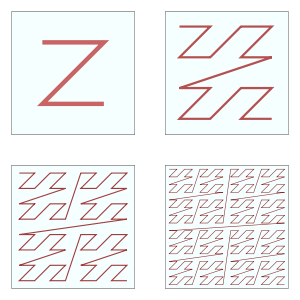
\includegraphics[width=0.7\linewidth]{zcurve}
		  		\caption{Space Filling Curve: Z Curve of order 1, 2, 3 and 4. Image source \cite{wiki:Zcurves} }
		  		\label{fig:zcurve}
		  	\end{figure}
		  
		  
		  \clearpage
		   \subsection{Geohash}
		   
		   Geohash is a system for geocoding Latitude and Longitudes to represent spatial coordinates in a compact String or Binary representation. It was invented by Gustavo Niemeyer in 2008. 		   \cite{wiki:geohash} \cite{Lee:2014:ESQ:2666310.2666481, 6691586} \cite{Balkic2012}
		   
		   In our work, we use  Geohash algorithms as hierarchical spatial data structure to partition geospatial big data based on the geographic region. Since the main focus of this work is partitioning, not indexing and we are dealing with points geometry Geohash is very useful. The algorithm controls data distribution in Spark by laying out data points to particular RDDs in the distributed clusters and also routing queries to specific RDD partition, allowing it to efficiently query few partitions.
		   
		   \subparagraph{Geohash as Hierarchical indexing structure}
		   
		   A Geohash code, in string format, represents a bounding rectangle grid on earth surface. Starting from resolution '1', Geohash string represents 
		   
		   Geohash algorithm partitions Earth into a 8 X 4 = 32 grids at each level and traverses through the grids in z-order \cite{wiki:Zcurves} to produce the encoded Geohash string. At Geohash resolution '1', the length of the Geohash string is '1', denoting the z position of the grid.
		   
		   These 32 grids in resolution '1' are further sub-divided into another 32 grids at Geohash resolution level '2' and making the two character long Geohash String. As the resolution of Geohash increases, the size of the grid(rectangular box) denoted by a Geohash String reduces making it more accurate in pointing to a particular place on earth. For instance, a Geohash of length '12' denotes a grid of 7cm\textsuperscript{2}.
			
				\begin{figure}[h]
				\centering
				\includegraphics[width=1.05\linewidth]{Geohash}
				\caption{Geohash grid of resolution '1' and '2'}
				\label{fig:Geohash}
				\end{figure}
						   
		   \clearpage
		   The below table \ref{tab:Geohash_Resolution} shows the dimensions of geohash cells for Geohash string lengths from 1 to 12. However, it is important to note that the dimensions of the cells varies from Equator to poles. 
		   \cite{elastic_geohash}
		   
		   \begin{table}[h]
		   	\centering
		   	\begin{tabular}[htbp]{llllc}
		   		\\	\hline 
		   		
		   		\textbf{GeoHash length}			&\textbf{Area width x height}  \\
		   		\hline
		   		1				&5,009.4km x 4,992.6km \\
		   		2				&1,252.3km x 624.1km \\
		   		3				&156.5km x 156km \\
		   		4				&39.1km x 19.5km \\
		   		5				&4.9km x 4.9km \\
		   		6				&1.2km x 609.4m \\
		   		7				&152.9m x 152.4m \\
		   		8				&38.2m x 19m \\
		   		9				&4.8m x 4.8m \\
		   		10				&1.2m x 59.5cm \\
		   		11				&14.9cm x 14.9cm \\
		   		12				&3.7cm x 1.9cm \\
		   		
		   		\hline
		   	\end{tabular}
		   	\caption{Geohash cell dimension for varied length of Geohash String(@Equator)}
		   	\label{tab:Geohash_Resolution}
		   \end{table}
		   
		   \subparagraph{Properties of Geohash: } \cite{Geohash}
		   \begin{enumerate}
		   	\item Geohashes could be used as Uniqur Identifiers and a representation of POint data in databases \cite{wiki:geohash}
		   \item As we remove characters from the right end of a Geohash string, it loses precision and covers a larger region.
		   \item Two Geohash strings with same prefix are closer to each other. However, the contrary is not true. Two Geohash strings with different prefix are nearby too. This is due to the longer Z curve distance between two grids in the Equatorial and Polar regions.
		   		   \item Exploiting the above property, Geohash index structure could be used for quick-and-dirty proximity search.
		   
		   \end{enumerate}
		   
		    All these properties of Geohash encoding system are exploited in designing a Geospatial Partitioning scheme in Apache Spark. 
		   
		   \clearpage
		   \subsection{Related Work} 
		   
		   Owing to the increased use cases for location aware data, many of the recent non-relational databases have focused on providing geospatial support by supporting spatial-indexing schemes. Geohash, out of the many schemes,  is used as indexing scheme by 
		   MongoDB \cite{MongoDB} and Apache Solr \cite{apachesolr}. 
		   
		   \textit{Geospark }\cite{geospark}, one of the projects from DataSys Lab at Arizona State University, extends Apache Spark to provide geospatial support and claims to exhibit better performance in comparison to its hadoop based implementation, SpatialHadoop \cite{spatialhadoop}. Geospark provides Spatial RDDs and Spatial operations on those RDDs. It allows to choose from R-Tree and Quad-Tree based indexing schemes. 
		   
		   The motto of our work is not to draw comparison with these systems. Our motto is to design a lightweight spatial partitioning scheme based on Geohash encoding technique, without much modification to internal implementation of Apache Spark. It is a high level design which is not restricted only to Spark and could be easily modified to use in any other distributed computing environment. 
		   
		  
     \cleardoublepage
     \hfill
	\section{GeoHash Partitioner: Design and Implementation}
		\hfill 
	
	In this chapter, we look into the design and implementation of a custom spark partitioner that provides  Geospatial partitioning of spatial big data
		\subsection{Partitioning}
			\par As we realize, communication is very expensive in a distributed environment, it is necessary to distribute data in a such a way that minimizes communication. This would result in performance gain and greatly improves speed of execution for key based transformations. In Geospatial application, this means, laying out RDD partitioning in such a way that retains spatial locality of the data points. 
			
			However, (Geospatial) Partitioning is not helpful (or not beneficial) in all applications and scenarios. The gain is considerable when: \cite{sparkbook}
			\begin{itemize}
				\item The dataset is scanned multiple times in key oriented operations like \textit{joins}.
				\item Considerable dataset size wherein benefits of partitioning outweighs the effort involved partitioning.
				\item And clearly when the application involves a relatively more spatial queries.
			\end{itemize}
			
		\subsubsection{Default Partitioning in Spark}
			\par Spark allows programs to take control over their RDD's partitioning and this configurable partitioning is provided only for RDDs of key-value pairs, for instance JavaPairRDD \cite{sparkapiPairRDD}, since special distributed "\textit{shuffle}" operations, such as grouping or aggregating the elements by a key.\\
			
				\begin{figure}[h]
					\centering
					\includegraphics[width=0.85\linewidth]{partitioning}
					\caption{Hash key based Partitioning scenario in Spark}
					\label{fig:partitioning}
				\end{figure}
				
			\clearpage
			\par Spark provides two default partitioning schemes:
			\subparagraph{HashPartitioner} partitions records based on their key's hash using Java's Object.hashCode method. The partition is obtained as,
			
			\begin{quote}
				\centering Partition = key.hashCode() / numPartitions
			\end{quote}
			
			\subparagraph{RangePartitioner} partitions sortable records by range into roughly equal ranges. The content of the RDD passed in are sampled to determine the range\cite{sparkapiPartitioner}. This partitioning scheme is useful when keys have natural ordering and are non-negative.
			
			Spark's \texttt{HashPartitioner} and \texttt{RangePartitioner} do not involve \textbf{domain specific knowledge} during partitioning. The absence of domain knowledge tends to hash the locations \textit{L1(40.881142 -73.907021)} and \textit{L2(40.88129 -73.90693)} into two different partitions even though these two locations are physically closer and are intended to stay within a single partition. However, Spark provides \textbf{Custom Partitioner object} to leverage domain specific(Geospatial) knowledge to further cut down communication cost. Rest of this segment demonstrates the design of a Geospatial aware custom Partitioner.
			
			\par It is important to note that during partitioning based on key, spark does not provide explicit control of which physical worker node each key goes to. This is partly because of the system design to support node failures.\cite{sparkbook} However, it ensure that the set of keys resides in the same partition. For instance, keys that produce same hashcode stick together  in the same partition. So, in our aim to achieve spatial locality with the data points we could achieve partition level locality, not node level i.e., the data points corresponding to the neighboring region, at a particular level of resolution, might physically reside in different nodes of the cluster. However all data points belonging to a 'same' region(containing same geohash prefix) reside within a single partition and in turn in the same physical node. So, we could summarize the properties of partitioning in Spark as follows: \cite{partitioningHeather} 
			 
			 \begin{enumerate}
			 	\item Each node in a spark cluster can contain one or more partitions
			 \item Partitions never span across multiple node. Records in a single partition are guaranteed to be in the same node.
			\item  The number of partitions in the RDD, \texttt{\textbf{numPartitions}} parameter, could be configured. Default value: Total number of cores on all executor nodes.
			 \end{enumerate}
			
		\paragraph{	Contract to implement a Custom Partitioner: }
			The implementation of Custom Partitioner should extend org.apache.spark.Partitioner class and implement the following three methods:\cite{sparkbook}
			
			\begin{itemize}
				\item \textbf{\texttt{numPartitions: Int}} - returns the number of partitions that will be created.
				\item \textbf{\texttt{getPartition(key: Any): Int}} - returns the partition ID (0 to numPartitions-1) for a given key.
				\item \textbf{\texttt{equals()}} - the standard Java equality method. When two RDDs are aggregated or operated on, Spark uses this method to verify the Partitioner object against other instance of Partitioner if both RDDs are partitioned the same way i.e., using the same custom Partitioner.
			\end{itemize}
			
		\subsection{Geohash as Partitioning Key}
			\par In the background section, the structure and usage of Geohash technique was discussed. Here we use Geohash as the key for creating our Key-Value RDD. We generate this Geohash key by encoding the Latitude and Longitude values from each record. \\
						
				\begin{figure}[h]
					\centering
					\includegraphics[width=0.3\linewidth]{GeohashEncoder}
					\caption{Geohash encoder to encode spatial points to Geohash Key}
					\label{fig:GeohashEncoder}
				\end{figure}
		In our approach, we use Geohash of Latitude, Longitude of each record as its key. We create a Key-Value RDD with the generated Geohash code as Key and the record itself as the value, as shown in table. 
		\begin{quote}
			Geohash Key = GeoHashEncode.withCharacterPrecision(Lat, Long, 12\footnote{12 - the  maximum precision of 12 characters for 64bits Geohash}).toBase32()
		\end{quote}
				\begin{figure}[h]
					\centering
					\includegraphics[width=0.85\linewidth]{kvrdd}
					\caption{Sample records of Key-Value RDD with Geohash code as key}
					\label{fig:kvrdd}
				\end{figure}
				
				As discussed in the background section of Geohash technique, this encoding scheme based on Z-curves, could be used in retaining spatial locality. All data points with same Geohash prefix belong to the same geographical region. This encoding scheme also helps in identifying neighbour along the path of the z traversal. So, the next step is create custom partitioner based on the Geohash code.

		
		\subsection{Custom Geohash Partitioner}
		
		\par The custom extension of Partitioner object should be able to read a record's key and assign a partition number specific to that particular key. Since we need to create spatial awareness to partition allocation we cannot utilize Java Hashcode method on the keys(Geohash) to determine its destined partition. Hence, our custom Geohash partitioner requires a mapping from desired Geohash grid to a physical partition number of the RDD. So, whenever there is an input record's key, the custom partitioner refers to mapping meta-data and returns destined partition number. The design and construction of the \textit{GeohashPartitionMapper} is explained in detail in the following sections.
		The approach is to leverage the inherent property of Geohashes to denote grids on the earth surface, to create the partitions. For instance, all of New York region falls under the grid 'd'. So, when we partition data from entire world and need all data points in New York and neighboring region to reside in the same partition then we map all Geohash key with prefix of length 1 as 'd' to the same partition number.  
		
		Key '\textit{dr5rugbmh6ym}', at geohash grid resolution 1 has the prefix 'd', goes to partition 'x'
		Now Key '\textit{dr5rusvvxq1d}', at geohash grid resolution 1 has the prefix 'd', also goes to partition 'x'
		Whereas the key '\textit{sr72w4ntct4y}' with 's' as grid resolution 1 prefix, goes to partition 'n', because physically the code represents a point in Europe, not NYC. The Geohash grid for the world with resolution size '1' is shown in Figure \ref{fig:Geohash_res1}
							
			\begin{figure}[h]
			\centering
			\includegraphics[width=0.7\linewidth]{img/Geohash_res1}
			\caption{Geohash grid of resolution '1'}
			\label{fig:Geohash_res1}
			\end{figure}
		
		To proceed further deeper and to denote smaller region as a partition size, we could simply increase the size of Geohash prefix considered as partition. This means drilling into Geohash grid resolution 2, wherein each of the 32 grids are in turn  sampled into another 8x4 grids(32 grids). This would result in a permutation of 32 x 32 = 1024, distinct partitions, Figure \ref{fig:Geohash_res2}. As the work proceeds with this approach, we are hit by the explicit side effect of Hashing techniques - imbalance in load distribution as seen in Graph \ref{fig:imbalance}. This is also prominent with spatial datasets with data point concentrated at hotspots, major cities and metropolitan areas. 
		
			\begin{figure}[h]
				\centering
				\includegraphics[width=0.7\linewidth]{img/Geohash_res2}
				\caption{Geohash grid of resolution '2'}
				\label{fig:Geohash_res2}
			\end{figure}
		
		
		At a particular Geohash grid resolution, amongst the 32 cells of a grid, if one grid represents a major city (hotspot), then the remaining 31 cells/partitions have very few data points and in turn result in idle processing time. Lets look into a smaller data set for points in Manhattan region:
		
		\begin{itemize}
			\item All data points have a common Geohash key prefix - '\textit{dr\dots\dots}' i.e., the complete Manhattan dataset is enclosed with Geohash grid resolution 2.
			
			\item So, in order to create Geohash key to Partitions mapping, we drill deep into grid resolution 3. It results in 32 possibilities[Geohash base32 code 0-9 b~z] from '\textit{dr0\dots\dots}' to '\textit{drz\dots\dots}' and hence 32 partitions. However, when we look at Figure \ref{fig:imbalance}, we realize that around 95\% resides in a single partition, 5\% in another, leaving out 30 empty partitions
				
			\item An attempt to balance load, by drilling deeper into one more resolution, would result in further increase starving partitions as shown in Figure \ref{fig:imbalance2}
		\end{itemize}
							
				\begin{figure}[hp]
					\centering
					\includegraphics[width=0.9\linewidth]{imbalance}
					\caption{Imbalanced distribution of elements into partitions}
					\label{fig:imbalance}
				\end{figure}		
				

				
				\begin{figure}[hp]
					\centering
					\includegraphics[width=1\linewidth]{imbalance2}
					\caption{Increase in number of empty (or) imbalanced partitions}
					\label{fig:imbalance2}
				\end{figure}
			
			\clearpage
		
		\begin{itemize}
			\item This imbalance continues to exist until we ignore the load distribution and blindly increase the overall resolution of the Geohash grid
			\item Extremely varied size of partitions would result in other spark executors waiting idly for tasks or in \textit{speculative execution} of tasks for slow running tasks. This is the behavior of spark to  transfer Map task from slower nodes to the nodes that have already finished processing their allocation \cite{sparkspeculation}. Or even worse hit time out on \texttt{spark.locality.wait} which would result in poor locality violating the core purpose of our partitioning. The effort to achieve \textit{process local} fails and task steps through process-local, node-local, rack-local and then any. \cite{sparkconfiguration}. However both these parameters could be controlled by configuration settings.
		\end{itemize}

		
			\subsubsection{Load Aware Geohash Key Generator}
				\par To avoid this phenomenon, our approach takes into consideration the geographical distribution of load and in addition leverages benefits of Geohashing to make balanced, location aware partitioning. The result would benefit both from (Geo)Hash based partitioning, to achieve locality, and from Range based partitioning, to attain maximum achievable (or) configured level of uniform load distribution. The custom partitioner achieves this by,
				 \begin{enumerate}
				 	\item Determining a threshold parameter based on the size of dataset.
				 	\item Drilling deeper into resolutions only for those grids which has number of data points greater than the calculated threshold.
				 	\item Stop partitioning on grids which has fewer points which would result in varied levels of resolution in different Geohash grid depending on the geographical load distribution.
				 
				 \begin{figure}[h]
				 	\centering
				 	\includegraphics[width=0.7\linewidth]{img/Geohash_res2_loadbalance}
				 	\caption{Geohash grids of varying resolution based on Load distribution}
				 	\label{fig:Geohash_res2_loadbalance}
				 \end{figure}		
				 
				 	\item Iterative process stops at the resolution when there are no further grids with more points than the threshold (or) at a pre-configured level of resolution. For our evaluation, we configured a maximum grid resolution depth of 6 levels.
				 	\item This varied resolution in areas is stored in a general (tree like or HashMap) data structure
				 \end{enumerate}
									 
							 
			
			\subsubsection{Algorithm}
			
			\paragraph{Encode the Coordinates}
				\begin{itemize}
					\item Create the key-value RDD, \textbf{JavaPairRDD}\textit{[String, Array[String]]}, with '\textit{Geohash of the coordinates}' in data-set as keys. This is the base RDD which is to be partitioned.
					\item Create a secondary RDD, with just the key from previous RDD. \textit{RDD[String]}. This reduced RDD, with only Geohash string, helps in reduced load during learning about load distribution and creating a Geohash grid to partition mapping. 
				\end{itemize}
			\paragraph{Determine the Threshold}
				The next step is determine the \textit{threshold}, which is considered as maximum number of records a region/grid could contain to stay in a single partition. Threshold is calculated in terms of average number of records each partition could handle within a default partition size. The approach chooses\textit{ number of records} as the threshold parameter because it might vary depending upon number and type of columns for different datasets.
				
				
				\begin{quote} Partitioning Threshold \footnote{Average Record in each partition}  = Total number  of records / Number of default partitions
				\end{quote}
				
				Total number of records counting is done alone with any operation that involves overall scan
			
			\paragraph{Deeper Resolution Tree building}
				The next step is to understand the load distribution w.r.t threshold. This is then used to build the data structure which contains mapping between Geohash Grid to partition number.
				
				\begin{itemize}
					\item Instantiate and maintain a new list to collect key prefix.
					
					\item From the KeyRDD, starting from the prefix size '1', count the number of elements in distinct keys (reduceByKey)
						\begin{quote} val level1 = keysRDD.map(a => (a.substring(0,1), 1)).reduceByKey(\_+\_ )
						\end{quote}
						
					\item From the result set, if value < threshold $\to$ add the current Geohash prefix to the list 
					
					\item For all values > threshold $\to$ increase the prefix size to '2' and again count the number of elements in distinct key
						\begin{quote} val level2 = keysRDD.map(a => (a.substring(0,2), 1)).reduceByKey(\_+\_ ) 
							 (for all 'a' not shortlisted in Level1)
							 
						\end{quote}
				 
					\item Repeat the count operation by increasing the length of the code by one character for every iteration until the predefined level of Geohash resolution or there are no segments that has more records than threshold. 
					\item When the desired final level is reached, do not filter based on threshold, instead add all the left out Key prefix to the list.
					\item This would involve 'n' times complete scan of dataset. So, to optimize it, we could create a \textit{reduceByKey} on the nth prefix length and calculating it in the reverse. This would involve only 1 complete scan of the data set. (n - the predefined prefix limit need to estimate load)
			 	
				\end{itemize}
															
				\begin{figure}[h]
					\centering
					\includegraphics[width=1\linewidth]{levels1}
					\caption{Levels of load distribution for increasing Geohash resolution}
					\label{fig:loadlevels}
				\end{figure}
			
			\clearpage						
				
			\paragraph{Variable length Key data structure}
				\par Finally the list would contain varying lengths of Geohash prefix. This variable length key could be stored in a tree data structure or a hashmap and each of them assigned a partition number. This would be the GeoHash partition mapper metadata and it is fed as input to our custom Geohash Partitioner for Spark. \\
			
					\begin{figure}[h]
						\centering
						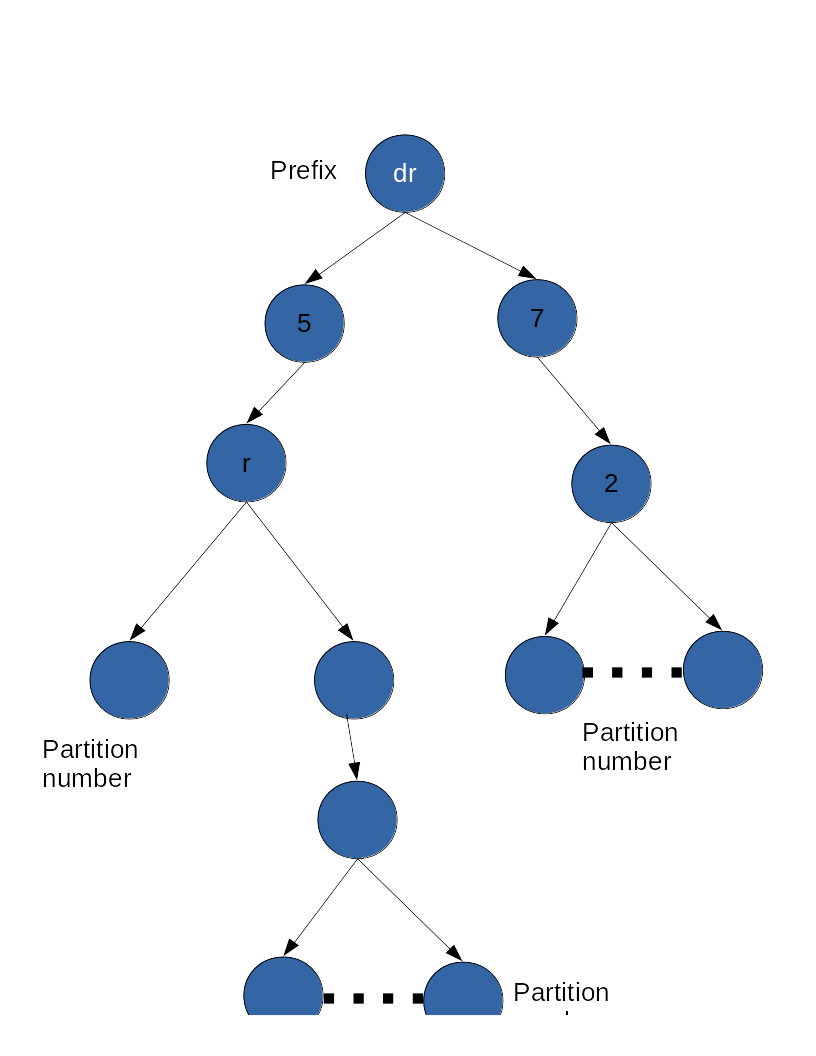
\includegraphics[width=0.8\linewidth]{key}
						\caption{Geohash Partition mapper: variable length load aware Geohash key data structure}
						\label{fig:keydatastrucutre}
					\end{figure}
			 \clearpage
			\paragraph{Optimized Partitions}
			The partitioner achieves good geo-load balancing by following above approach. However, there is scope for further optimization. Consider the scenario where we have two different Geohash Prefix of same length and number of elements in one Geohash Prefix exceeds the threshold. In this case, the procedure is to retain the prefix with less elements than threshold and drill deeper into the other prefix. This would result in 32 new partitions in the additional resolution. However if only one among these 32 contributed to more than 90\% of its parent prefix's total number of elements, then this leaves other 31 under fed partitions which could have otherwise been combined into a single partition, see Figure \ref{fig:Optimization}, \ref{fig:Optimization2}
									
				\begin{figure} [h]
				\centering
				\includegraphics[width=0.7\linewidth]{img/Optimization}
				\caption{Enhanced optimization in creating Geohash Partitioning}
				\label{fig:Optimization}
				\end{figure}
			So, we further enhance the algorithm to combine neighboring Geohash prefixes that could stay well as in a single partitions as demonstrated in the Figure \ref{fig:Optimization4}.		
			
			\paragraph{Persistence after Custom Partitioning}		
			Once a huge data set is partitioned based on any custom partitioner, it is necessary to persist the resulting RDD, either in memory or disk. If the RDD is not persisted, the subsequent usage of this RDD would result in repeated custom partitioning and involve reevaluation of the RDD's complete lineage. Hence failure to persist this RDD would nullify the benefits of \texttt{partitionBy()}, by incurring repeated partitioning and shuffling of records across the cluster. This would have been the case of not using any partitioner. \cite{sparkbook}
			
			\clearpage	
						
			\begin{figure}[p]
			\centering
			\includegraphics[width=0.7\linewidth]{img/Optimization2}
			\caption{Geohash Partition 'e' is further partitioned to deeper resolution(has only 3 hotspot partitions)}
			\label{fig:Optimization2}
			\end{figure}
						
						
			\begin{figure}[p]
			\centering
			\includegraphics[width=0.7\linewidth]{img/Optimization4}
			\caption{Previously under-fed 28 partitions combined and reduced to 3 joint partitions}
			\label{fig:Optimization4}
			\end{figure}
			
			\clearpage
			\subsection{Architecture Overview}
				\par The below architecture diagram gives an overview of all the components in Geohash based load aware partitioner \\
				\begin{figure}[h]
					\centering
					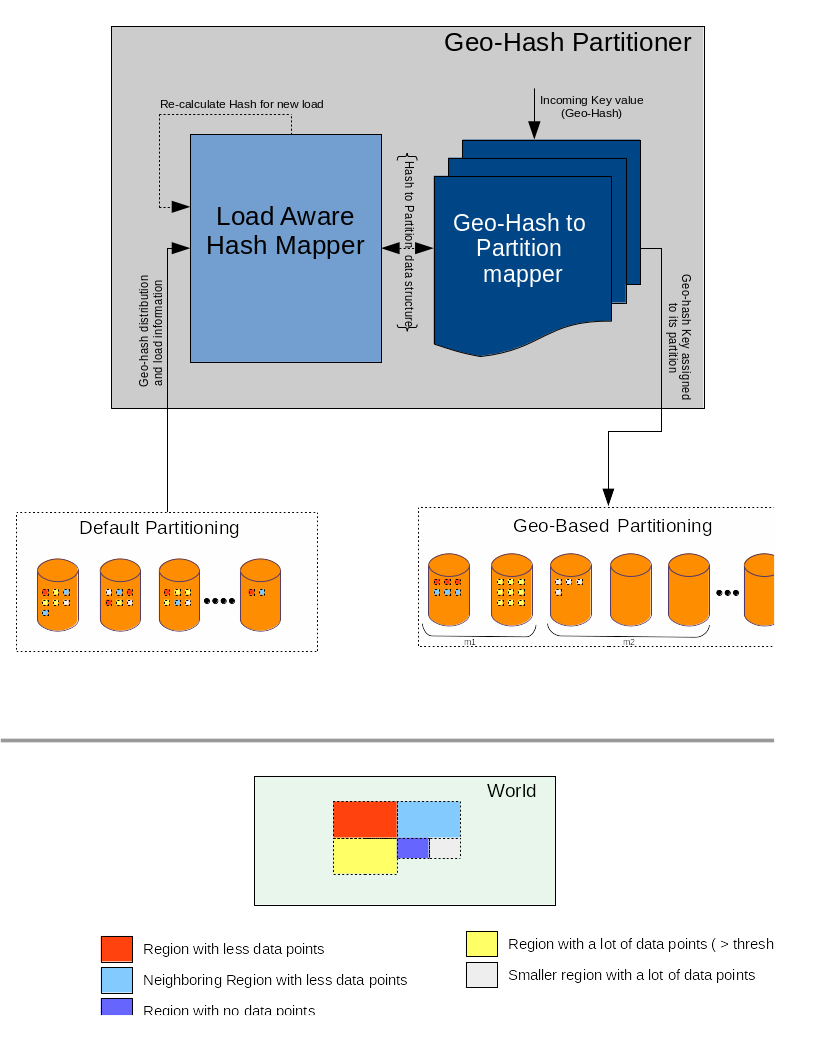
\includegraphics[width=0.81\linewidth]{img/Architecture}
					\caption{Architecture Overview: Geohash Partitioner}
					\label{fig:Architecture}
				\end{figure}
				
			
			
	  \cleardoublepage
	\hfill
	\section{GeoHash Query Optimizer: Design and Implementation}
	\hfill
	
		\par In this chapter, we look into the design and implementation of the Query Layer that leverages knowledge from Geohash Partitioning to perform efficient querying 
		\subsection{Partition Pruning}
			\par After running Geohash based partitioning of our dataset, subsequent operations on the resultant RDD would result in reduced network communication. Moreover, the application has a clear knowledge on the partitioning logic - how the dataset is partitioned and in which specific partition the data for a particular region resides.
			
			The general behavior of spark is that whenever there is an incoming tasks, it is launched on all partitions. For instance, when there is filter to extract all the restaurants in Chicago, the filtering task in launched on all the partitions even on the ones which holds records only from Australia. Now that the application has control on partitions based on the custom Geohash partitioner, we could leverage this knowledge to affect only those partitions which are of our concern. 
			
			
				\begin{figure}[h]
				\centering
				\includegraphics[width=0.65\linewidth]{img/Queryonallnodes}
				\includegraphics[width=0.65\linewidth]{img/Queryonallnodes2}
				\caption{Spark's default behavior to launch tasks in all partitions}
				\label{fig:Queryonallnodes2}
				\end{figure}
				
				Spark provides an api, \textbf{\texttt{PartitionPruningRDD<T>}}, which is an RDD used to prune existing RDD partitions in order to prevent launching tasks on all partitions \cite{sparkapiPartitionPruning}. This helps us to launch tasks only on partitions that are of concern for the filter operation in the execution DAG. 
				
									
					\begin{figure}[h]
					\centering
					\includegraphics[width=0.7\linewidth]{img/partitionprunning}
					\caption{Spark Partition Pruning RDDs launching tasks on selected partitions}
					\label{fig:partitionprunning}
					\end{figure}
					
					Our approach builds a Query Translator to translate incoming queries into geographic region and in turn use these regions to pick potential candidate partitions, based on the information from Geohash Partition mapper, previously built for partitioning. We then build a query optimizer module which prunes the candidate partitions and launches tasks on these smaller subset of partitions.
									
		\subsection{Geohash Query Translator}
		
		\par The purpose of this module is to analyze the incoming task or query and mark down the regions of interest for that particular query. In the following section, we shall take a look into how the translation works when we have a spatial '\textbf{\textit{Within}}' query (say, show me all the restaurants \textit{150 meters} from \textit{here})

			\begin{itemize}
				\item This type of query provides us with the point of interest\textit{(p)} and the desired distance\textit{(d)}.
				\item In our approach, we make use of spatial distance calculation function like \textit{Haversine formula} \cite{wiki:Haversine_formula} (or) \textit{Vincenty's formulae} \cite{wiki:Vincenty's_formulae} in our distance calculation between any two points on the earth.
				\item From the point of interest, calculate a circle(c) with a radius of the d. This query circle(c) is created by all points that are a distance d  from the point of interest(p). 
				\item Using this query circle, a minimum bounding box that completely covers circle of interest  is calculated. The mathematical formula for calculating bounding box coordinates are derived from \cite{HandbookofMathematics} and clearly explained in the work \cite{matuschek_2010}
			
			\end{itemize}		
				\clearpage	
				\begin{figure}[h]
				\centering
				\includegraphics[width=1.0\linewidth]{img/QueryOpt0}
				\caption{Query translated into Bounding Box for region of interest}
				\label{fig:QueryOpt0}
				\end{figure}
					
			 
			Now query has been translated into a bounding box and this query bounding box contains all the data points that are of interest to us. The coordinates of this derived bounding box is fed as input by the next module, \textbf{\textit{Geohash Query Optimizer}}, to pick candidate partitions to run the tasks on.
			
		\subsection{Geohash Query Optimizer}
		
			\par Identifying partitions corresponding to Query Bounding Box, pruning them from the Geohash partitioned RDD and launching the tasks on them is the purpose of Geohash Query Optimizer. The bounding box is evaluated against the Geohash Partition mapper to determine the list of partitions. The details of this procedure as listed below:
			
			\begin{itemize}
				\item The query bounding box has four coordinates and these are encoded into their respective Geohash string.
				\item The longest common prefix is calculated from the four coordinates' Geohash. This prefix covers all the Geohashes of the data points that are required for this query. 
				
					\begin{table}[h]
						\centering
						\begin{tabular}[htbp]{llllc}
						\\	\hline 
							NorthWest:           & \textbf{dr5r}uj4477kd       \\
							SouthWest:          & \textbf{dr5ru}46ne2ux       \\
							SouthEast:          & \textbf{dr5ru}6ryw0cp     \\ 
							NorthEast:          & \textbf{dr5ru}mpfq534     \\ \hline 
							Query Bounding Box Prefix: & \textit{\textbf{dr5ru}}\\
							\hline
						\end{tabular}
						\caption{Query Bounding Box Prefix}
						\label{tab:Query Bounding Box Prefix}
					\end{table}
				
				\item The prefix is evaluated against the key values in Geohash Partition mapper and all the matching partition numbers are retrieved as depicted in Figure \ref{fig:PruningPartitions}
			\end{itemize}
			
				\clearpage	
					\begin{figure}[p]
					\centering
					\includegraphics[width=0.7\linewidth]{img/QueryOpt2}
					\caption{Translating Query into Regions of interest(Bounding Box)}
					\label{fig:QueryOpt2}
					\end{figure}
				
			
					\begin{figure}[p]
						\centering
						\includegraphics[width=1.0\linewidth]{img/PruningPartitions}
						\caption{Choosing partitions to prune based on Query Bounding Box prefix}
						\label{fig:PruningPartitions}
					\end{figure}		
			
		\clearpage
			\subsubsection{Enhanced Optimization}
				\par This candidate partition section procedure could be further optimized by efficiently ignoring partitions that are within the query bounding box prefix but out of Query circle. This could be achieved by taking advantage of the knowledge about varied levels of Geohash grid resolution and dropping out partitions that are not needed for the query as shown in the Figure \ref{fig:QueryOpt3}. As we could see, only \textit{4 out of 32} inner partitions of grid '\textit{\textbf{k}}' are of interest for this query and so the remaining 28 partitions could be easily dropped from consideration. Bigger grids, grid '\textit{\textbf{7}}', with no further inner partitions has to be considered as whole.
				
				
					\begin{figure}[h]
					\centering
					\includegraphics[width=0.7\linewidth]{img/QueryOpt3}
					\caption{Enhanced candidate partitions selection based on varied grid resolution information}
					\label{fig:QueryOpt3}
					\end{figure}
			
			Once the candidate partitions are identified by using either of these methods, they are pruned out from the large partitioned RDD and task is launched on the resulting, pruned RDD as shown in Figure \ref{fig:partitionprunning}. This results in a much lesser workload and reduced scans needed to obtain the same results and in turn enhances performance. The efficiency of \textit{Geohash Partitioning and Query optimizing} approach could be evidently noticed from the evaluation results. The following section shows the results of evaluation for the test cases run on New York Taxi Data.
			
		 
		\clearpage
		
		\subsection{Architecture Overview}
			The below architecture shows the complete components of the Geohash based Query optimizer \\
			\begin{figure}[h]
				\centering
				\includegraphics[width=0.9\linewidth]{img/Architecture2}
				\caption{Architecture Overview: Geohash Query Optimizer}
				\label{fig:Architecture2}
			\end{figure}
		
  \cleardoublepage
  
  \hfill
  \section{Evaluation and Results}
  \hfill
  		  \subsection{System Footprint}
		  
				\begin{figure}[h]
				\centering
				\includegraphics[width=1.0\linewidth]{SystemFootprint}
				\caption{Apache Spark clusters running on Top of HDFS}
				\label{fig:system-footprint}
				\end{figure}
		  
		  \subsection{Results}
		  \hfill
		  \subsection{Challenges and Limitations}
		  \par The default hash partitioning algorithm in spark depends on Java hash code. For every incoming record, the hash code of its key is generated. Each hash code which is an integer, is mapped on to one the available partitions using 
		  \begin{quote}
		  	Partition number = Hashcode / No.of partitions. 
		  \end{quote}
		  In this case, the hashcode to partition mapping is always calculated dynamically.
		  
		  However, in our case, since hashcode is a geohash string and we perform a load balanced hash partitioning we always need the data structure that holds the load aware geohash to RDD partitions mapping metadata. We need this metadata to perform partitioning. As
		  
  \cleardoublepage
  
  \hfill
  \section{Conclusions}
  \hfill
		   \subsection{Contributions}
	   	   \subsection{Future Work}
	   	   
	   	   \par Our dissertation concerns mainly about Geometry Points. This could be extended to support composite Geometries like LineString, Polygons, Circles which would represent Transport routes, city boundary, travel zones respectively.
	   	   Once partitioning is completed the
   	  
   	   
  \cleardoublepage
 
 \clearpage
 
 %=====BIBLIOGRAPHY================================================================================
 \bibliographystyle{ieeetr}
 \bibliography{GeoHashPartitionerReference}	  

\end{document}
